\chapter{A Data Acquisition System for the Test Beam}
\label{chap:II-3-test-beam}

  During the ongoing process of the development of the DAQ system, the electronics has been tested in two test beams organised in Fall 2014 and Fall 2015. The first test beam, ran with the first prototype of the DAQ, aimed at proving the feasability of the architecture of the system, not focusing on data taking from the provided pion and muon beam but rather on usability. As the results were encouraging, the second version of the electronics was developped involving a complete redesign of the hardware, firmware, and software. Therefore, we will mainly focus on the second test beam, which electronics is described in the previous chapter, during which abundant data was recorded showing both excellent results for the detectors and the DAQ system. \\

  In this chapter, we present the firmware and software developments done for the DAQ system for the test beams followed by the analysis of the recorded data. First, we will present the firmware architecture of the OH and the GLIB to better understand the global layout of the system and the features that have been implemented to control the components. Then we will move on to the back-end applications developped to control and monitor the DAQ system and read out data. Finally, after a presentation of the layout of the test beam setup and its characteristics, we will show the results obtained after analysis of the recorded data.

  \section{Architecture of the OptoHybrid Firmware}

    The most important function of the OptoHybrid is to transfer data between the VFAT2s and the GLIB. Downwards, from the off-detector to the on-detector electronics, it transfers slow control requests and fast commands while upwards it sends the trigger and tracking data back to the back-end system. Next to the handling of the basic VFAT2 functionnalities, it must also handle the optical links and a couple of programmable registers which control the system. Furthermore, procedures that were previously implemented in software and required extensive computanionnal time have been moved to firmware in order to speed up the system. \\

    Although rather complex, the firmware of the OptoHybrid can be decomposed in six blocks: the fast commands, the trigger data, the tracking data, the slow control, the calibration routines, and the optical links. Eventough these blocks separatly will be presented, they are tighlty interconnected using a wishbone-like architecture for intercommunication.

    \subsection{Internal Communication Through a Wishbone-Like Architecture}

      Wishbone is an open-source communication protocol used in many projects to enable data transfer between ICs. A light version of the protocol has been implemented in the OptoHybrid to link the various modules of the system. The latter are divided in two categories: masters which initiate requests, and slaves which provide responses. The link between the two is done through a switching hub which redirects the requests to the appropriate slaves by using a 32-bit-long address space mapped to the various modules. By design, multiple masters can interact simultaneously with different slaves allowing for parrallelism in the system. \\

      A request form a master is composed of four signals: a flag signaling the presence of a request, a write-enable bit to indicate the nature of the request (read or write), a 32-bit-long address to which the request will be redirected, and an optionnal 32-bit-long data field in case the request is a write operation. The response from a slave consists of: an ackownledgment signal, a 4-bit-long error status in case the operation failed, and an optionnal 32-bit-long data field holding the response to read requests. A programmable timeout has also been implemented to avoir blocking operation. Some components implement both a master and a slave module in order to be able to receive requests and propagate them to various other modules. \\

      Communication done through the wishbone-like protocol is used mainly for slow control or non-time-critical operations as the latency of a transaction is not fixed. Indeed, the switching hub implements a waiting list functionnality which allows two masters to address the same slave at the same time by storing one of the requests in memory and awaiting for the slave to finish the other transaction.

    \subsection{Encoding Fast Commands}

      Fast commands such as L1As, Resyncs, BC0s, etc can originate from various sources. In normal data taking runs, the AMC13 receives the TTC signals, forwards them to the microTCA AMC which in turn transmits them to the OptoHybrid. When data taking is stopped and calibration runs are performed, the routines implemented in the OptoHybrid are ran and require fast commands. To this end, the TTC signals can also be generated locally using the T1 generator block. This entity can generate L1As, Resyncs, BC0s, and CalPulses in three different ways: send a single command a given number of times at fixed interval, send a CalPulse followed by a L1A with a fixed delay, or send a programmable pattern involving all the commands. Finally, the two remaining sources of TTC commands, and more precisly L1As, are either a loopback from a given VFAT2 trigger bits directly to all the VFAT2s (self-triggering) or the signals coming from an external component through a debugging header on the OptoHybrid. \\

      The switching between the various sources is done by setting a register through slow control operations. Once the source has been selected, the commands are forwarded to the VFAT2s and encoded on the T1 signals. Each command is composed of three bits clocked at 40 MHz. An additionnal feature has been added to the L1A line to throttle the trigger signals when working in high rate environments. Through registers, the operator can select to send only a fraction of the received commands to not overload the VFAT2 buffers and allow for correct readout of the chip.

    \subsection{Formatting Trigger Data}

      Each of the 24 VFAT2s transmits eight trigger bits per BX. These are regroupped using a logic OR in the DAQ system of the test beam  thus yielding 24 bits. The trigger information is used for calibration routines and forwarded over debugging headers to an external electronics crate. As the number of external connections is limited, only six trigger bits can be send thus requiring the need for a selection mechanism controller by programmable registers.

    \subsection{Acquiring Tracking Data}

      Upon reception of a L1A, the VFAT2 transfers the selected event from its SRAM1 to SRAM2 and then to an encoder which serialises the data. Each event is 192 bits long followed by two idle bits and clocked at 40 MHz. This means that it takes 194 BXs to read out one event and that the VFAT2 cannot handle trigger rates higher than $\approx$ 200 kHz without experiencing an overflow of the buffers. The data is pushed out of the VFAT2 automatically and formatted according to the pattern shown in Figure \ref{fig:II-3-test-beam-vfat2-tk-format}. The top left bits are Most Significant Bits (MSBs) which are pushed out first and the bottom right bits or the Least Significant Bits (LSBs) which come in last. The first four bits of the first three 16-bit-long words are constant values. These are completed by the BC which increments at each clock cycle, the EC which counts the number of received L1As, four flags which hold information on the status of the buffers, and a chip ID unique to each VFAT2. Following are the 128 bits reflecting the hit information on each channel. Finally, the VFAT2 uses a Cyclic Redundancy Check (CRC) on 16 bits to detect errors. The CRC uses all other 176 bits to encode its data but does not provide a way to correct errors. \\

      \begin{figure}[h!]
        \centering
        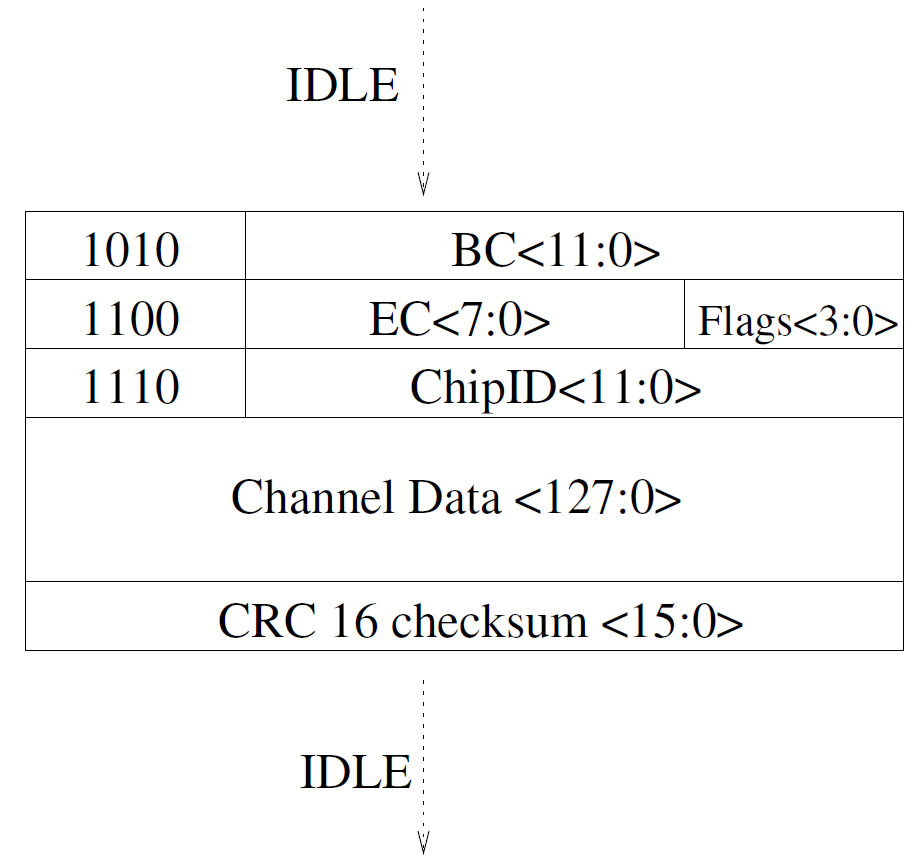
\includegraphics[width=0.5\textwidth]{img/II-3-test-beam/vfat2-tk-format.png}
        \caption{??? \cite{Aspell:1069906}.}
        \label{fig:II-3-test-beam-vfat2-tk-format}
      \end{figure}

      Next to the data line, each VFAT2 provides a DataValid line which is pulled high when the bits coming out of the VFAT2 are valid. However, due to the limited number of pins connecting the GEB and the OptoHybrid, this signal has been left unconnected for all but six VFAT2s. Therefore, data is constantly shifted in a 194 bits (192 bits of data and 2 idle bits) serial-to-parrallel converter and analyzed. When the fixed pattern of 12 bits is seen, a flag is raised signaling the presence of potential data. The data packet is split up in its various elements and the CRC is recomputed and compared against the received CRC. Two additionnal flags respectivly hold the results of the comparation of both CRCs indicating if the data is valid or not, and a logic OR of all 128 channel to indicate if the packet contains a hit or not. In theory, only packets with valid CRCs could be transmitted to the back-end electronics. However, sending all packets offer the possibility to identify recurring errors in the CRCs computation and offers the possibility to correct them offline. \\

      In parallel to the decoding of the data packets, the OptoHybrid maintains its own BC and stores the value of the counter in a buffer each time a L1A is received. When the decoding modules report they have detected data, a concentrator module aggragates the information from all available VFAT2s. Every packet received within a window of 10 BX is assigned to the same event to which the value of the corresponding BC is appended. The assembled event is stored in a large buffer to be latter sent over the optical links to the GLIB. \\

      To prevent positions either not equipped with VFAT2 Hybrids or that are noisy to generate fake data, a 24-bit-long register allows to mask individual positions to ignore any packets it generates. Next to this, each decoding module is equipped with two counter respectivly counting the number of valid and invalid packets.

    \subsection{Controlling and Monitoring the Systems}

      The OptoHybrid is used to control itself through wishbone and the VFAT2s through I2C. The slow control of the OptoHybrid mainly consists in selecting TTC command sources, setting the trigger throttling, reading out counters, etc. These operations are performed to control the data flow and the functionning of the DAQ system itself. Commands sent to the VFAT2s on the other hand have direct impact on the physics of the data taking through the biais of the analog front-end readout. \\

      To communicate with the VFAT2s, six I2C controllers are implemented in the firmware of the OptoHybrid, one per sector on the GEB. Each controller can access four VFAT2s which are identified using three resistors that can be installed on the GEB. VFAT2 uses a modified I2C protocol which uses the same frame format as the official one but a different addressing scheme. The official I2C data frame is shown in Figure \ref{fig:II-3-test-beam-i2c}. The master starts by sending seven address bits which are used to identify the slave it wants to talk to, followed by a read/write bit. After the slave acknowledged the request, eight bits are sent from the master to the slave in case of a write operation followed by a slave acknowledgment, or the opposite in case of a read operation. For the VFAT2, the first three bits of the address are used to select the chip that is addressed by the master while the four remeaning bits are used to select the register that needs to be accessed. This addressing scheme allows the OptoHybrid to access up to 16 registers on the VFAT2s. However, each VFAT2 holds 16 primary registers and 136 extended registers. The extended registers are accesses using two primary pointer registers: one set to point to an extended register, and one to read/write the data in said register. Thus, in order to perform a transaction on a primary register, only one operation is necessary, while two are required to access extended registers. \\

      \begin{figure}[h!]
        \centering
        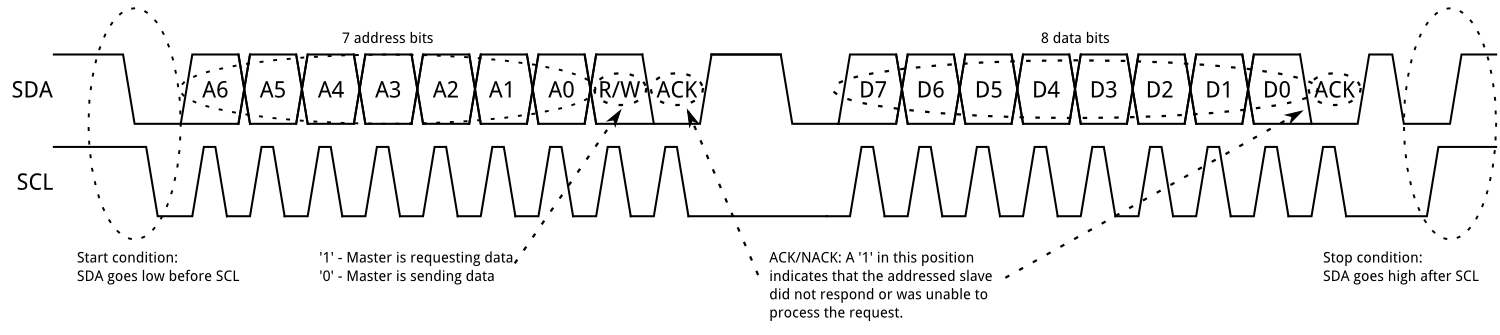
\includegraphics[width=\textwidth]{img/II-3-test-beam/i2c.png}
        \caption{??? \cite{I2C}.}
        \label{fig:II-3-test-beam-i2c}
      \end{figure}

      To make this process transparent to the user and flatten out the address space of the VFAT2s, the OptoHybrid maps the primary registers from addresses 0 to 16 and the extended registers from addresses 17 to 152. When performing a transaction with the extended registers, the I2C controllers automatically run the double addressing scheme. \\

      Next to the basic I2C controllers, an extended I2C controller was developped to abstract individual addressing and allow request broadcasting. This module forwards I2C requests to all selected VFAT2s at once to configure the entire system in parallel. A programmable register allows to leave out given VFAT2s from the broadcast while a buffer stores the result of the operations.

    \subsection{Calibrating the Systems}

      The calibration routines have been ported from software to firmware in order to increase their speed of operation and reduce the number of requests that need to be performed. The routines are as follows: a threshold scan which measures the noise on the strips as a function of the threshold of the VFAT2s, a latency scan which allows to select the correct BX when receiving L1As, and a s-curve scan which characterize the response of the strips as a function of the collected charge and threshold. \\

      \paragraph{The threshold scan} is used to scan each VFAT2 for noise. For each threshold value set on the VFAT2, the percentage of events displaying a hit is recorded and taken as the percentage of noise. A graph can be obtained showing the noise decrease as the threshold increases yielding a point at which the system can be operated with minimal noise. The threshold scan can be operated using trigger information on the 128 strips as a whole or on individual strips using tracking data. For the latter, the T1 generator is used as trigger source to generate data as these runs being performed when the beam is off. No relation between a L1A and physical event is needed to study the noise on the system. \\

      \paragraph{The latency scan} allows to determine the best latency value to be set in a VFAT2. The latency is the time difference, in number of BX, between the time of arrival of a L1A and the time at which the related event was stored in the VFAT2 buffer. This module is operated when the particle beam is on and triggers are generated by an external source such as a Photomultiplier (PM) placed in front of the detector. For each value of the latency, the OptoHybrid counts the ratio of events with hits over the total number of events. For a noiseless VFAT2 with 100\% detection efficiency, the ratio would be 0\% outside the correct latency window and 100\% inside. The size of the window can be adjusted by changing the length of the monostables output in the VFAT2s. \\

      \paragraph{The s-curve scan} is part of the calibration routines performed for the qualification of the VFAT2s. It yields the response of the VFAT2 strips to an injected charge pulse according to the threshold. It is used in conjunction with the T1 generator which send a CalPulse followed by a L1A at fixed interval, thus with known latency. The use and results obtained for this module are further detailled in Chapter \ref{chap:II-5-qualification}.

    \subsection{Optical Communication with the Off-Detector Electronics}

      The link between the OptoHybrid and the off-detector electronics are the optical links from which two are used: one for the trigger data and fast commands, and one for the tracking data and slow control. Each link can transfer 64 bits per BX in both directions.

  \section{Architecture of the GLIB Firmware}

  \section{The Control and Monitoring Application}

  \section{The Test Beam Setup}

  \section{Analysis of the Collected Data}



























  -
